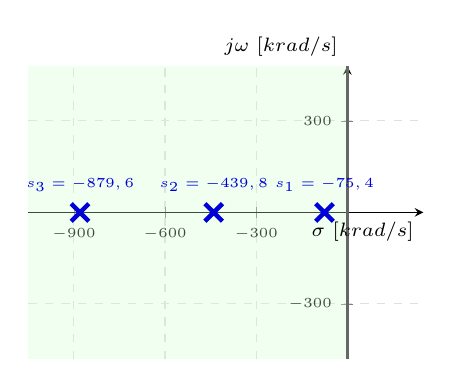
\begin{tikzpicture}
  \begin{axis}[
    width=6.6cm, height=5.3cm,
    axis lines=middle,
    xlabel={$\sigma$ [$\text{krad/s}$]},
    ylabel={$j\omega$ [$\text{krad/s}$]},
    xlabel style={at={(ticklabel* cs:1)}, anchor=north east, font=\scriptsize},
    ylabel style={at={(ticklabel* cs:1)}, anchor=south east, font=\scriptsize},
    xmin=-1050, xmax=250, ymin=-480, ymax=480,
    xtick={-900, -600, -300},
    ytick={-300, 300},
    grid=both, grid style={gray!25, dashed},
    tick label style={font=\tiny},
  ]
    % Zona estable LHP sombreada sutilmente
    \fill[green!20, opacity=0.3] (axis cs:-1050,-480) rectangle (axis cs:0,480);

    % Eje jw (frontera de estabilidad)
    \draw[line width=1.0pt, black!60] (axis cs:0,-480) -- (axis cs:0,480);

    % Polos de G(s)
    \addplot[only marks, mark=x, mark size=4.5pt, line width=1.6pt, blue!85!black]
      coordinates {(-75.40, 0) (-439.82, 0) (-879.65, 0)};

    \node[above=4pt, blue!85!black, font=\tiny\bfseries] at (axis cs:-75.40, 0) {$s_1 = -75,4$};
    \node[above=4pt, blue!85!black, font=\tiny\bfseries] at (axis cs:-439.82, 0) {$s_2 = -439,8$};
    \node[above=4pt, blue!85!black, font=\tiny\bfseries] at (axis cs:-879.65, 0) {$s_3 = -879,6$};
  \end{axis}
\end{tikzpicture}
